%---------------------------------------------------------------------------------
\chapter{Introduction} \label{chp:introduction}
%---------------------------------------------------------------------------------

Over the last decade kernel based learning methods are one of the most popular research topics in machine learning. According to a statistic\footnote{http://learning.eng.cam.ac.uk/zoubin/talks/ICML-Presentation.pdf}, ``kernel" is one of the most popular keywords in ICML conference since 1988.A number of kernel machines, e.g., support vector machines (SVMs)~\cite{ml/CortesV95}, kernel Fisher discriminant (KFD) ~\cite{nn/MikaRWSM99}, and kernel
principal component analysis (KPCA) ~\cite{neco/ScholkopfSM98}, have been proposed and become state-of-the-art methodologies. These approaches have shown practical relevance not only for classical classification and regression problems but also, in clustering, dimensionality reduction, etc. Kernel based learning algorithms have been successfully applied to a wide range of applications in various fields, such as pattern and object recognition, text categorization, time-series prediction, finance, gene expression profile analysis, DNA and protein analysis, etc. Some good surveys on kernel machine learning topics can be found in ~\cite{datamine/Burges98,tnn/MullerM01,Scholkopf2002,ss/MoguerzaM06}.

The key idea of kernel methods can be briefly explained as follows~\cite{as/HofmannSAS08}. Classically, theories and algorithms of machine learning and statistics have been very well developed for the linear case. However, real world data analysis problems often require nonlinear methods to detect the kind of dependencies that allow successful prediction of properties of interest. By using a positive semi-definite (PSD) kernel, one can sometimes have the best of both worlds. The kernel corresponds to a dot product in a (usually high-dimensional) feature space. In this space, our estimation methods are linear, but as long as we can formulate the computation in terms of kernel evaluations, we never explicitly have to compute in the high-dimensional feature space.

The kernel function plays a central role in kernel machines. Empirical evidence shows that the performance of a kernel method relies more on the kernel function rather than the kernel machine. For example, kernelized logistic regression, kernelized regularized least square, and support vector machine often result in similar performance. Most of the off-the-shelf algorithms have been kernelized if they could be. Therefore, how to design or learn a good kernel has become an important research topic in machine learning research.

In this chapter, we introduce kernels informally as similarity measures that arise from a particular representation of patterns. The goal is to provide an overview of the basic concepts. Then we describe the problem of {\em kernel learning} and summarize our contributions. Finally we give organization and some notation table.

%===========================================================
\section{Preliminaries}
%===========================================================

Supervised classification is one of the fundamental problems of learning theory: Suppose we are given two classes of objects. We are then faced with a new object, and we have to assign it to one of the two classes. This problem can be formalized as follows: we are given empirical data $(\x_1,y_1),\ldots,(\x_n,y_n)\in\mathcal X\times\{+1,-1\}$. Here, $\mathcal X$ is some nonempty set from which the patterns $\x_i$ (sometimes called cases, inputs, instances, observations, points or samples) are taken, usually referred to as the {\em domain}; the $y_i$ are called {\em labels, targets, outputs} or sometimes also {\em observations}. Note that we only consider two classes of patterns, +1 and -1 respectively. This simple situation is referred to as {\em binary classification}.

It should be emphasized that the patterns are just abstraction which could be about anything, and we have not made any assumptions on $\mathcal X$ other than it being a set. For instance, the task might be to categorize sheep into two classes, in which case the patterns $\x_i$ would simply be sheep.
In order to study the problem of learning, however, we need an additional type of structure. In learning, we want to be able to generalize to unseen data points. In the case of pattern recognition, this means that given some new pattern $\x\in\X$, we want to predict the corresponding $y\in\{\pm1\}$. By this we mean, loosely speaking, that we choose $y$ such that $(\x, y)$ is in some sense similar to the training examples. To this end, we need notions of similarity in $\X$ and in $\{\pm1\}$. It is easy to characterize the similarity of the outputs $\{\pm1\}$: in binary classification, there are only two situations can occur: two labels can either be identical or different. The choice of the similarity measure for the inputs, however, is a deep question that lies at the core of the field of machine learning.

Let us consider a similarity measure of the form
\begin{eqnarray}
&k:&\X\times\X\rightarrow\R\nonumber\\
&&(\x,\x')\mapsto k(\x,\x')
\end{eqnarray}
that is, a function that, given two patterns $\x$ and $\x'$, returns a real number characterizing their similarity. Unless stated otherwise, we will assume that $k$ is {\em symmetric}, that is, $k(\x,\x')=k(\x',\x)$ for all $\x,\x'\in\X$. For reasons that will become clear later, the function $k$ is called a {\em kernel}.

General similarity measures of this form are rather difficult to study. Let us therefore start from a particularly simple case, and generalize it subsequently. A simple type of similarity measure that is of particular mathematical appeal is a {\em dot product}. For instance, given two vectors $\x, \x'\in\R^d$, the canonical dot product is defined as
\[
\langle\x,\x'\rangle:=\sum_{i=1}^dx_ix_i'.
\]
here $x_i$ is the $i$th component of $\x$. The geometric interpretation of the canonical dot product is that it computes the cosine of the angle between the vectors $\x$ and $\x'$, provided they are normalized to length 1. A similarity function plays a central role in learning. For example, with a well defined kernel $k$, one can use nearest neighbor for classification, i.e., the label of a test point $\x$ is predicted as the label of its nearest neighbor in the training set. Furthermore, we can compute the average similarity between $\x$ and the positive/negative training set.

With the similarity function $k$, one can proceed on devising learning frameworks. Among the large volume of classification algorithms, {\em support vector machine} is one of the most influential techniques. Refer to \cite{Scholkopf2002} for a more detailed introduction.

%=========================================================
%\section{Why Kernel Learning?}
\section{Motivation: Why Kernel Learning?}
%=========================================================

A large volume of works on kernel design/learning has emerged and exhibited strengths in a variety of applications in the machine learning community. In the standard framework of kernel methods, the choice of an appropriate kernel is left to the user and a poor selection may lead to sub-optimal performance. Moveover, empirical evidence shows that the performance is often dominated by the kernel being used rather than the type of the kernel machine. Therefore, how to choose or design or learn a ``good" kernel is a crucial problem. Instead of using a fixed kernel function, sample points can be used to select or construct a kernel function/matrix suitable for the learning task.

The focus of this thesis is how to learn a kernel from data, either a closed-from kernel function or a kernel matrix (the value of each entry is the kernel evaluation result). In the sequel, we do not distinguish kernel function from kernel matrix if it is clear in the context. Informally, the problem of {\em kernel learning} is to devise a closed-form kernel function, or construct/learn the kernel matrix on a sample $\mathbf X$ (typically in the transductive setting), given an accessible sample of data (both labeled and unlabeled), a prior kernel, or any form of useful prior information to help to determine the kernel.

The kernel is the prior knowledge we have about a problem and its solution. Accordingly, just as there is no ``free lunch" in learning, there is also no free lunch in kernel choice. Kernel learning is very challenging and still under exploration. First, a kernel has to guarantee the positive definiteness, which is a necessary constraint to make the kernel valid. This is often difficult to justify. The resultant optimization problem is often very difficult to solve, for example, learning the kernel matrix is in nature a semidefinite program\cite{Boyd}. Second, the design of good kernel requires deep insights about the problem at hand, for instance, the manifold structure of the data. We know that the kernel essentially maps the data into a high-dimensional space. However, this property does not provide semantic hints on which kind of kernels are useful for classification. Third, it calls for theories that connect the kernel and the error risk on test data such that the learning of kernel is principled and essentially effective. Due to these difficulties, kernel learning is still being actively studied.

Researchers have proposed various methods on this topic. One approach is to construct kernels based on known ones guided by some general tricks. A successful work is Multiple Kernel Learning (MKL), which learns a convex combination of some basic kernels (e.g., \cite{jmlr/LanckrietCBGJ03}). Another scheme is to specify a parametrization of the kernel based on some insights of the problem (e.g., \cite{icml/KondorL02}). Recently, nonparametric kernel learner has emerged to learn a kernel matrix directly from training data with few assumptions on the kernel structure (e.g, \cite{jmlr/TsudaRW05}\cite{icml/KulisSD06}\cite{icml/HoiJL07}\cite{icml/LiYW07}). In chapter 2, we conduct a thorough survey on background knowledge and recent advances on representative kernel learning methods.

%=========================================================
\section{Problems and Research Scope}
%=========================================================

In general, our research focus in this thesis is about to design and develop {\em effective} and {\em efficient} kernel learning algorithms. More formally, the general problem can be described in the following.

{\em Given a set of training samples (possibly together with side information), how to learn an effective kernel for classification, clustering, or data embedding efficiently?
}

Specifically, this thesis aims to tackle the above  challenge by the following approaches:
\begin{itemize}
  \item to study efficient non-parametric kernel learning (NPKL) algorithms. Unlike parametric MKL algorithms, the variables to be solved in NPKL is a positive semi-definite matrix, which is usually very hard to solve. A typical interior-point solver for NPKL has the time complexity of $O(N^{6.5})$, which makes NPKL prohibitive for large-scale real applications;
  \item To explore new heuristics for designing more effective multiple kernel learning (MKL) algorithms. Most existing MKL algorithms follow the same optimization framework as SVM. Despite being studied extensively, their empirical performance is not always satisfied. We aim to study more effective MKL algorithms beyond the SVM-based framework.
\end{itemize}

Besides the investigation of novel algorithms, another important research scope of this thesis is to examine the efficacy of kernel learning techniques when be applied to solve some challenging problems in real-world applications. Specifically, this thesis will explore kernel learning techniques to tackle challenges in two important real applications: (i) image re-ranking task in social image retrieval, and (ii) social strength modeling task in social media community mining. We have conducted extensive experiments on large-scale real datasets to validate the efficacy of the proposed solutions.



%=========================================================
\section{Summary of Contributions}
%=========================================================

The major contributions of this thesis include:
\begin{itemize}
  \item We conduct a thorough survey on both the foundations of kernel machines and recent development of kernel learning, including concepts, algorithms and theories. We believe such a survey with consistent notations and organizations are valuable;
  \item We propose a family of non-parametric kernel learning (NPKL) algorithms, named SimpleNPKL, which avoids semi-definite programming in traditional NPKL methods, such that NPKL can be significantly boosted to handle data set of 10K samples. The framework is general enough to apply to classification, clustering, and data embedding tasks;
  \item We explore two novel directions of multiple kernel learning algorithms (MKL): {\em deep} MKL and {\em unsupervised} MKL, beyond the traditional SVM based and kernel target alignment based principles. Empirical results on public available data sets shows the proposed directions are promising;
  \item We apply kernel learning techniques to solve two important applications: image re-ranking and social strength modeling, and conduct extensive sets of empirical studies on large-scale real datasets.
\end{itemize}

In next section, we introduce the organizations of the thesis. Readers can jump to the part of their particular interest.



%=========================================================
\section{Thesis Organizations}
%=========================================================

In chapter 2 we introduce the basic concepts and theories on kernel machines and statistical machine learning. We first give formal definitions on positive definite kernel and related concepts (RKHS). Then we describe the most popular kernel method--support vector machine and related work on kernel learning. To provide deep insights on such traditional supervised learning algorithms, we also discuss the classical statistical learning theory. Since optimization techniques have already tightly intertwined with machine learning research. We introduce the general form of convex problems and {\em semi-definite program} (SDP). After that we describe the transductive learning problem with insights. Our SimpleNPKL framework is a natural recipe in this problem setting. It avoids heavy computation cost of SDP and yields satisfactory performance in transductive learning.

%With these necessary background knowledge, we conduct a survey on various kernel learning methods in chapter 3. Classical multiple kernel learning (MKL) algorithms are described in a detailed manner as it is seminal of kernel learning. Then we restrict our attention to non-parametric kernel learning algorithms, where efficiency perspective is the core we discuss. Besides that we pay special attention to the generalization risk of kernel learning, which is complementary to current efficiency oriented MKL methods.

In chapter 3, we propose a family of Simple Non-Parametric Kernel Learning (SimpleNPKL) algorithms for efficient and scalable non-parametric kernel learning.  With our new solution, the NPKL can be solved efficiently. Therefore, NPKL is made as a practical learning scheme for real application. We conduct extensive experiments, which show that SimpleNPKL is significantly more efficient than existing NPKL methods. We extend the proposed SimpleNPKL scheme to resolve other non-parametric kernel learning problems, including {\em colored maximum variance unfolding} \cite{nips/SongSBG07}, {\em minimum volume embedding} \cite{aistats/ShawJ07}, and {\em structure preserving embedding}\cite{icml/ShawJ09}. The encouraging results show that our technique is able to speed up the existing non-parametric kernel learning solutions significantly for several real-world applications.

In chapter 4 and 5, we explore two novel directions towards more effective kernel learning algorithms, beyond the traditional linear multiple kernel combinations in SVM framework. The former one is deep MKL, inspired by recent research in deep learning, while the second is unsupervised MKL, inspired by recent advances in local coordinate coding techniques. We evaluate these techniques on several publicly available datasets.

In chapter 6 and 7, we apply kernel learning (parametric or non-parametric) algorithms to two important applications: image re-ranking and social strength modeling on multimedia platforms. Empirical results verify both the efficiency and effectiveness of our techniques in real applications.

In the last chapter, we make the conclusion of this thesis and discuss future directions towards improving kernel learning.

\begin{figure}\label{fig:organization}
\begin{center}
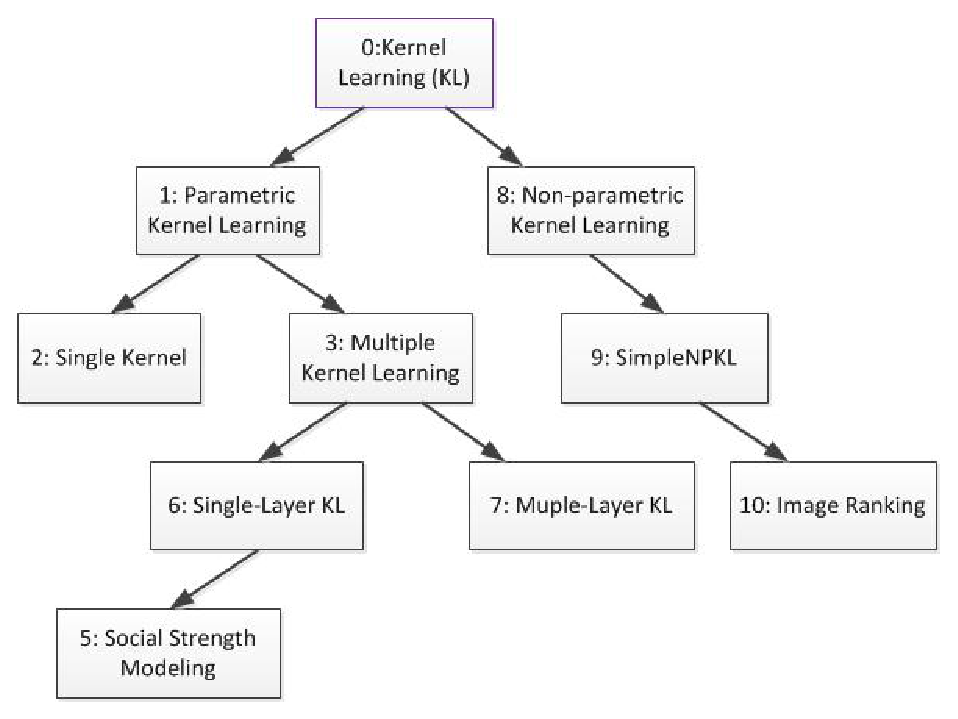
\includegraphics[width = \linewidth]{figures/organization.eps}
\caption{Organization on the topic kernel learning.}
\end{center}
\end{figure}

To summarize, Figure \ref{fig:organization} presents a high-level organization of this thesis. Our contribution can be categorized into the nodes in this figure. Specifically, 
\begin{itemize}
  \item 9: chapter 3 presents a fast algorithm for non-parametric kernel learnring, SimpleNPKL;
  \item 7: Chapter 4 presents a deep multiple-layer multiple kernel learning framework;
  \item 5: Chapter 7 presents an application of MKL for social strength modeling;
  \item 6: Chapter 5 presents an unsupervised MKL foramework;
  \item 10: Chapter 6 presents an image ranking framework with the idea of non-parametric kernel learning, using the idea of SimpleNPKL.
\end{itemize}

%=========================================================
\section{Notation Table}
%=========================================================

To make the rest presentation clear, we give the common notations in Table \ref{table:notation} and common abbreviations in Table \ref{table:abbreviation} for reference.

In the whole thesis, we use bold upper case letters to denote matrix, bold lower case letters to denote vector, and curlicue letters to denote a vector space (could be for training samples, decision functions, etc.).

\begin{table}[!ht]
\centering \caption{Some common notations used in the thesis. } \label{table:notation}
\begin{center}

\begin{tabular}{ll}
\hline
\hline
Notation &Explanation\\
\hline
$\mathbb R$ &domain of real number\\
$\mathbb N$ &domain of negative integer\\
$\mathbb S^n_+$ &$n$-dimensional symmetric positive semi-definite matrix\\
%$\mathbb I(c)$  & returns 1 if $c$ is true and 0 otherwise\\
%$[n]$ & $:=\{1, \ldots, n\}$\\
$\X$ &domain from which the samples come from\\
$\mathbf X$ & a set of points\\
$\x$  &a single point, typically belonging to $\mathbb R^d$\\
$x_i$ &the $i$th component of $\x$\\
$y$   &the label of $\x$, taking value $\pm1$ in binary classification case\\
$\x^\top$ &transpose of $\x$\\
$\langle \x, \x' \rangle$ &$:=\x^\top\x'$, inner product between vectors (matrix)\\
$\x_i\circ\x_j$ &element-wise multiplication between vectors (matrix)\\
$k$   &kernel function\\
$\Phi$  & the implicit mapping function of some kernel $k$\\
$\mathbf K$   &kernel matrix, the value of $(i,j)$ entry is the evaluation $k(\x_i,\x_j)$\\
$\tr \mathbf K$ & the trace of the matrix $\mathbf K$\\
$\| \mathbf K\|_F$ &the Frobenius norm of the matrix $\mathbf K$\\
%$d$ &dimensionality of the data\\
%$n$ &number of labeled points\\
%$u$ &number of unlabeled points\\
$f$   &a decision function defined on $\X$\\
%$l$ &a loss function defined on $\mathbb R$, typically the input is $yf(\x)$\\
%$P(A)$ &the probability of event $A$ happens\\
%$\mathbb E_x(A)$ &the expectation of $A$ over $x$\\
%$\mathcal F$  &the space to which the solution $f$ exist\\
%$\mathcal H$  &hypothesis space\\
$\mathcal H_K$ &Hilbert space induced by some kernel $\mathbf K$\\
\hline
\end{tabular}
\end{center}
\end{table}


\begin{table}[!ht]
\centering \caption{Some common abbreviations used in the thesis. } \label{table:abbreviation}
\begin{center}
\begin{tabular}{ll}
\hline
Abbreviation &Explanation\\
\hline
\hline
SVM & support vector machine\\
KL  & kernel learning\\
MKL & multiple kernel learning\\
$L_p$-MKL & $L_p$-norm regularized MKL\\
NPKL & non-parametric kernel learning\\
DMKL & deep multiple kernel learning\\
UMKL & unsupervised multiple kernel learning\\
%SKL &supervised kernel learning\\
%KTA & kernel target alignment\\
SDP & semi-definite programming\\
PSD & positive semi-definite\\
PDS & positive definite and symmetric\\
%IR & information retrieval\\
SSM & social strength modeling\\
\hline
\end{tabular}
\end{center}
\end{table}





